\chapter{Variablen, Datentypen \& Debugging}\label{ch:K03_Variables_Debugging}

\section{Variablen}
\begin{myexample}\label{myexample:ersteVariable}
In \cref{myexercise:Flaggen} haben Sie bereits die (quadratische) Flagge des Kantons Zürich mithilfe der Turtle gezeichnet. Ohne Beachtung der Farben könnte der Code dafür wie in \cref{listing:ohne_variable} aussehen.

\lstinputlisting[language=Python,caption=\texttt{ohne\_variable.py},label=listing:ohne_variable]{Grundlagen_Info/00_Programmieren/Skript/Code/K03_Variables_Debugging/ohne_variable.py}

Angenommen wir wollten die Grösse der Züri-Flagge ändern, dann müssten wir den Wert \pythoninline{50} an genau \textbf{drei Stellen} entsprechend anpassen! Dieses Vorgehen ist zum einen Mühsam und zum Andern höchst fehleranfällig (es kann sehr gut passieren, dass eine Änderung nicht konsequent an allen Stellen durchgeführt wird).

Viel besser ist es, wenn wir der Seitenlänge des Quadrats einen Namen geben. Genau dies haben wir in \cref{listing:mit_variable} getan: Wir haben der Länge den Namen \pythoninline{laenge} gegeben.
\lstinputlisting[language=Python,caption=\texttt{mit\_variable.py},label=listing:mit_variable]{Grundlagen_Info/00_Programmieren/Skript/Code/K03_Variables_Debugging/mit_variable.py}
Der Ausdruck \pythoninline{laenge} ist ein Beispiel einer sogenannten \textbf{Variable}.
\end{myexample}

\begin{mydefinition}[Variable in Python]
Eine \textit{Variable} in Python ist im Wesentlichen ein Name, der auf einen im Speicher (des Computers) abgelegten Wert verweist. Mit der Zuweisung
\begin{lstlisting}[numbers=none]
        a = 436 # a verweist auf ein Objekt vom Typ "ganze Zahl" mit dem Wert 436
    \end{lstlisting}
wird veranlasst, dass der Variablename \pythoninline{a} zu einer Referenz (einem Verweis) auf den Speicherort eines Objekts vom Typ \enquote{ganze Zahl} mit dem Wert \pythoninline{436} wird.
\end{mydefinition}

Eine Variable wird erstellt, sobald man ihr mit dem Gleichheitszeichen (\pythoninline{=}) ein Objekt zuweist. Das Gleichheitszeichen hat allerdings nicht dieselbe Bedeutung wie in der Mathematik! Vielmehr bedeutet das Gleichheitszeichen in Python: \enquote{die linke Seite ist ein Name für das Ding auf der rechten Seite}:
\begin{center}
	$ \tikzmarknode{b}{\text{\texttt{a}}} =\tikzmarknode{a}{\color{red}\underbrace{\color{black}\text{\texttt{10+3}}}}$
	\tikz[remember picture, overlay]{\draw[-latex,red] ([yshift=0.1em]a.south) to[bend left] ([yshift=-0.3em]b.south);}
\end{center}

Die Erklärung dieser Zeile ist: \enquote{Wir werten den Ausdruck \lstinline|10 + 3| aus und erhalten die Zahl 13. Diesen Wert (\lstinline|13|) speichern wir nun in der Variable \lstinline|a|}.

Wir können dies einfach überprüfen, indem wir den Wert von \lstinline|a| ausgeben:

\begin{lstlisting}
a = 10 + 3
print(a) # gibt 13 aus

a = 25 # der Wert der Variable wurde neu definiert
print(a) # gibt 25 aus
\end{lstlisting}

Variablen sind kurz gesagt ein Wort, das einen veränderbaren ($=$ variablen) Wert enthält. Der Variablenname darf dabei (fast) frei gewählt werden, sofern folgende Regeln eingehalten werden:

\begin{myoverview}[Benennung von Variablen]
	Bei der Wahl eines Variablennamens gibt es einige Punkte zu beachten:
	\begin{enumerate}
		\item Der Name muss mit einem Buchstaben beginnen (nicht: \verb|1meinname, _abc|).
		\item Der Name darf kein von Python \href{https://www.programiz.com/python-programming/keyword-list}{reserviertes Wort} sein (\lstinline|def, if, for| etc.).
		\item Der Name sollte \textbf{sinnvoll} und \textbf{beschreibend} (deskriptiv) sein. Wenn Sie beispielsweise die Höhe eines Hauses in einer Variable speichern, ist es sinnvoll, diese \lstinline|h| oder \lstinline|hoehe| zu nennen und nicht etwa \lstinline|x|.
		\item Variablennamen dürfen nur alphanumerische Symbole (\texttt{a--z, A--Z, 0--9}) und Unterstriche enthalten. Insbesondere also weder Leerzeichen noch Umlaute.
		\item Da Variablennamen keine Leerzeichen enthalten dürfen, sollten zusammengesetzte Namen mithilfe von Unterstrichen (\lstinline{_}) gebildet werden:
		      \begin{lstlisting}
                laenge_rechteck = 100
                number_of_occupied_squares = 5
            \end{lstlisting}
	\end{enumerate}
\end{myoverview}

\begin{myattention}
	In der Mathematik bedeutet das Gleichheitszeichen \enquote{der rechte Teil der Gleichung ist gleich dem linken}. Dies ist in Python nicht so! Hier bedeutet das Gleichheitszeichen: \enquote{werte den rechten Teil aus und \textbf{speichere} das Resultat im linken Teil}. Es gibt also \textit{keine} Speicherung von Werten in Python ohne Verwendung des Gleichheitszeichens.
\end{myattention}


\begin{myexercise}\label{ex:arithm-ausdruecke}
	Berechnen Sie die folgenden Ausdrücke in Python und speichern Sie das Resultat jeweils in einer Variable:
	\begin{table}[H]
		\centering
		\begin{tabular}{c|c}
			Berechnung      & Name der Variable \\\midrule\midrule
			$17 - 3 * 8$    & \texttt{res1}     \\\midrule
			$(5-2) * 4 + 1$ & \texttt{res2}     \\\midrule
			$3^6$           & \texttt{res3}     \\\midrule
			$18^{(2+3)}$    & \texttt{res4}
		\end{tabular}
	\end{table}
	\begin{myanswer}
		\lstinputlisting[language=Python,caption=\texttt{arithmetic\_vars.py},label=listing:arithmetic_vars]{Grundlagen_Info/00_Programmieren/Skript/Code/K03_Variables_Debugging/arithmetic_vars.py}
	\end{myanswer}
\end{myexercise}

\begin{myexercise}\label{ex:austausch}
	Sie wollen zwei Variablen Austauschen und kommen auf folgende Idee:
	\begin{lstlisting}[numbers=left]
        x = 5 
        y = 11
        # nun wollen wir die Werte austauschen, 
        # so dass y den Wert 5 und x den Wert 11 hat
        x = y
        y = x
\end{lstlisting}
	Führen Sie das Programm aus und geben Sie die Werte von x und y auf der Konsole aus. Funktioniert das Programm wie erwartet? Weshalb (nicht)?
	\begin{myanswer}
		x und y haben nun beide den Wert 11. Auf Zeile 4 wird der \textit{Wert} von y in x gespeichert. Ab diesem Moment haben sowohl die Variablen x wie y denselben Wert 11.
	\end{myanswer}
\end{myexercise}

\begin{myexercise}\label{ex:austausch-fix}
	Wie könnte der Code aus \cref{ex:austausch} angepasst werden, sodass er funktioniert?
	\begin{myanswer}
		Mit einer Hilfsvariable:
		\begin{lstlisting}
            x = 5 
            y = 11
            # nun wollen wir die Werte austauschen, 
            # so dass y den Wert 5 und x den Wert 11 hat
            temp = x # Hilfsvariable, um vorigen Wert von x zu speichern
            x = y
            y = temp
        \end{lstlisting}
	\end{myanswer}
\end{myexercise}

\section{Teilen mit Rest}
In diesem Abschnitt werden wir einige Überlegungen anstellen, welche Sie vielleicht an Ihre Zeit in der Primarschule zurückerinnern werden.
\begin{myexample}\label{myexample:teilenMitRest}
\leavevmode
\begin{itemize}
	\item Angenommen seit einem gewissen Zeitpunkt seien 23 Tage vergangen. Der Zeitpunkt liegt also 3 ganze Wochen zurück und in der vierten Woche sind bereits 2 Tage vergangen.
	      Wir können die Zahl 23 darstellen als $\textcolor{Red}{23} = \textcolor{Blue}{7}\cdot \textcolor{Green}{3} + \textcolor{Magenta}{2}$. Dabei ist $\textcolor{Green}{3}$ (der Quotient) das Resultat der \textbf{ganzzahligen Division} von $\textcolor{Red}{23}$ (Dividend) geteilt durch $\textcolor{Blue}{7}$ (Divisor). Dabei bleibt ein \textbf{Rest} von $\textcolor{Magenta}{2}$.
	\item Bei der ganzzahligen Division $\textcolor{Red}{23}$ geteilt durch $\textcolor{Blue}{7}$ bestimmen wir also, wie häufig $\textcolor{Blue}{7}$ vollständig (ganz) in  $\textcolor{Red}{23}$ \enquote{passt}.
	\item Nehmen wir weiter an, der Tag 0 sei ein Montag. Dann war auch schon Tag $-7$ ein Montag und ebenso Tag $+7$.
	      Offensichtlich entsprechen zwei Tage genau dann demselben Wochentag, wenn ihre Differenz (die Differenz ihrer Nummern) durch 7 teilbar ist\footnote{Mit anderen Worten: Ihre Differenz ist ein ganzzahliges Vielfaches von 7.}.
	      So sind beispielsweise die Tage 23 und 37 beide Mittwoche.
\end{itemize}
\end{myexample}

\begin{mydefinition}[ganzzahlige Divsion und Modulo-Operation (informell)]
Es seien $a$ und $b$ natürliche Zahlen und $b\neq 0$.
\begin{itemize}
	\item Wir bezeichnen in Python mit \lstinline{a // b} das Resultat der ganzzahligen Division von \lstinline{a} geteilt durch \lstinline{b} (wie oft hat \lstinline{b} ganz in \lstinline{a} Platz).

	      \textcolor{Gray}{Beispiel: \texttt{23 // 7} ist \texttt{3}.}
	\item Mit \texttt{a \% b} (sprich: \texttt{a} \textbf{modulo} \texttt{b}) bezeichnen wir den Rest, welcher bei der ganzzahligen Division von \lstinline{a} geteilt durch \lstinline{b} bleibt. Wir nennen \texttt{\%} die \textbf{Modulo-Operation}.

	      \textcolor{Gray}{Beispiel: \texttt{23 \% 7} ist \texttt{2}.}
\end{itemize}
Für mehr Details zur Division mit Rest siehe \cref{sec:DivisionMitRest}.
\end{mydefinition}

\begin{myexample}
Beispiele für die ganzzahlige Division in Python:
\begin{lstlisting}
20 // 3 # ist 6
80 // 4 # ist 20
37 // 5 # ist 7
\end{lstlisting}
\end{myexample}

\begin{myexample}
Beispiele für Modulo-Berechnungen (Rest der ganzzahligen Division) in Python:
\begin{lstlisting}
8 % 3 # ist 2
8 % 4 # ist 0
9 % 5 # ist 4
5 % 9 # ist 5
\end{lstlisting}
\end{myexample}

\begin{myexercise}\label{ex:modulo}
	Füllen Sie die zweite Spalte \textbf{von Hand aus}, berechnen Sie danach (zur Kontrolle) die Werte in Python.
	\begin{table}[H]
		\centering
		\begin{tabular}{r|l}
			\textbf{Code}     & \textbf{Resultat} \\\midrule\midrule
			\lstinline|1 % 3| & \lstinline|?|     \\\midrule
			\lstinline|2 % 3| & \lstinline|?|     \\\midrule
			\lstinline|3 % 3| & \lstinline|?|     \\\midrule
			\lstinline|4 % 3| & \lstinline|?|     \\\midrule
			\lstinline|5 % 3| & \lstinline|?|     \\\midrule
			\lstinline|6 % 3| & \lstinline|?|     \\\midrule
		\end{tabular}
	\end{table}
	\begin{myanswer}
		\begin{table}[H]
			\centering
			\begin{tabular}{r|l}
				\textbf{Code}     & \textbf{Resultat} \\\midrule\midrule
				\lstinline|1 % 3| & \lstinline|1|     \\\midrule
				\lstinline|2 % 3| & \lstinline|2|     \\\midrule
				\lstinline|3 % 3| & \lstinline|0|     \\\midrule
				\lstinline|4 % 3| & \lstinline|1|     \\\midrule
				\lstinline|5 % 3| & \lstinline|2|     \\\midrule
				\lstinline|6 % 3| & \lstinline|0|     \\\midrule
			\end{tabular}
		\end{table}
	\end{myanswer}
\end{myexercise}

\begin{myexercise}\label{ex:modulo-pizza}
	Berechnen Sie, wie viele Pizzastücke übrig bleiben, wenn \texttt{p} Personen an ein Fest kommen und eine Pizza mit \texttt{s} Stücken bestellt wird und jede Person genau gleich viele Stücke erhalten soll, indem Sie den Modulo-Operator verwenden. Testen Sie Ihren Code für unterschiedliche Werte \texttt{p} und \texttt{s}.
	\begin{myanswer}
		\lstinputlisting[language=Python,caption=\texttt{modulo\_pizza.py},label=listing:ModPizza]{Grundlagen_Info/00_Programmieren/Skript/Code/K03_Variables_Debugging/modulo_pizza.py}
	\end{myanswer}
\end{myexercise}


\begin{myexercise}\label{ex:modulo-gerade}
	Wie könnte berechnet werden, ob eine Zahl \texttt{z} gerade ist?
	\begin{myanswer}
		Wenn die Zahl \texttt{z} modulo 2 als Resultat 0 ergibt, ist die Zahl \texttt{z} gerade.
	\end{myanswer}
\end{myexercise}


\section{Werte von Variablen verändern}
Betrachten Sie das folgende Programm:
\begin{lstlisting}
    a = 10
    print(a) # a hat den Wert 10
    a + 5 # berechnet die Summe 10 + 5
    print(a) # a hat immernoch den Wert 10

    a += 7 # erhöhe den Wert von a um 7
    print(a) # hat nun den Wert 17
\end{lstlisting}
Es existiert also ein fundamentaler Unterschied zwischen den beiden Ausdrücken \pythoninline{x + 5} (Berechnung eines Wertes \textit{ohne} Speichern) und \pythoninline{x += 5} (Berechnung eines Wertes \textit{mit} Speichern).

\begin{table}[H]
	\centering
	\begin{tabular}{c|p{6cm}}
		\textbf{Befehl}        & \textbf{Bedeutung}                                                                                                         \\\hline
		\pythoninline{x += y}  & erhöht den Wert von \pythoninline{x} um \pythoninline{y}                                                                   \\\hline
		\pythoninline{x -= y}  & verringert den Wert von \pythoninline{x} um \pythoninline{y}                                                               \\\hline
		\pythoninline{x *= y}  & multipliziert den Wert von \pythoninline{x} mit \pythoninline{y} (und speichert das Resultat in \pythoninline{x})          \\\hline
		\pythoninline{x /= y}  & dividiert den Wert von \pythoninline{x} durch \pythoninline{y} (und speichert das Resultat in \pythoninline{x})            \\\hline
		\pythoninline{x //= y} & dividiert ganzzahlig den Wert von \pythoninline{x} durch \pythoninline{y} (und speichert das Resultat in \pythoninline{x}) \\\hline
		\pythoninline{x \%= y} & berechnet die Zahl \pythoninline{x \% y} (und speichert diese Zahl in \pythoninline{x})
	\end{tabular}
\end{table}

\begin{myexercise}\label{ex:spirale-increment}
	Zeichnen Sie eine Spirale der Form:
	\begin{figure}[H]
		\centering
		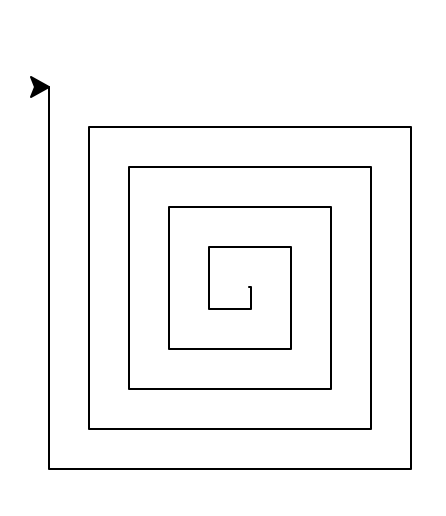
\includegraphics[width=0.3\linewidth]{Grundlagen_Info/00_Programmieren/Skript/Figures/spiral}
	\end{figure}
	Die Seitenlänge der Spirale soll nach jeder 90-Grad-Rotation um 10 länger werden.
	\begin{myanswer}
		\lstinputlisting[language=Python,caption=\texttt{spirale.py},label=listing:spirale]{Grundlagen_Info/00_Programmieren/Skript/Code/K03_Variables_Debugging/spirale.py}
	\end{myanswer}
\end{myexercise}

\begin{mysubmission}
	Geben Sie die Kubikzahlen von $1, 2, 3, \ldots, 10$ aus. Die Kubikzahl einer Zahl \texttt{x} ist gleich der Zahl hoch 3, also $\text{\texttt{x}}^3$. Die Kubikzahl von 1 ist demanch $1^3 = 1$ , die Kubikzahl von 2 ist $2^3 = 8$, etc.

	Geben Sie also die Zahlen $1 \;(=1^3), 8 \;(=2^3), 27 \;(=3^3), \ldots, 1000 \;(=10^3)$ aus, indem Sie eine Variable \texttt{x} verwenden, die am Anfang den Wert 1 hat und bei jeder Schleife um 1 vergrössert wird.
	\begin{myanswer}
		\lstinputlisting[language=Python,caption=\texttt{zahlen\_kubik.py},label=listing:kubik]{Grundlagen_Info/00_Programmieren/Skript/Code/K03_Variables_Debugging/zahlen_kubik.py}
	\end{myanswer}
\end{mysubmission}


\section{Arbeiten mit Text}

In Python kann man nicht nur Zahlen addieren, sondern auch mit Text arbeiten. In der Informatik verstehen wir unter einem \textit{Text} jede endliche Folge von Symbolen der Tastatur. Eine solche Folge von Symbolen bezeichnet man auch als \textit{Zeichenkette}\index{Zeichenkette} (Englisch: \textit{string}\index{string!Zeichenkette}). Ein einfaches Beispiel einer Zeichenkette haben wir bereits in \cref{myexample:prints} gesehen. Wir können Strings, ebenso wie Zahlen, in Variablen speichern.

\begin{myexample}\label{ex:text-in-variables}
Folgendes Beispiel speichert den Text \lstinline|"Hello, World!"| in der Variable \texttt{a}, der Wert der Variable wird danach auf der Konsole ausgegeben.

\begin{lstlisting}
a = "Hello, World!"
print(a)  # druckt auf der Konsole den Text "Hello, World!"
\end{lstlisting}
\end{myexample}

\subsection{Verkettung und Vervielfachung von Strings}
Zeichenketten können verkettet, also aneinandergehängt werden:
\begin{lstlisting}
    wort = "Kan" + "tons" + "schule"
    print(wort) # Kantonsschule
\end{lstlisting}
Die \enquote{Addition} von Strings wird \textit{Konkatenation}\index{Konkatenation} (Englisch: \textit{concatenation}) genannt.

Strings können mithilfe des \pythoninline{*}-Operators vervielfacht werden:
\begin{lstlisting}
    wort = "abc"
    print(4 * wort) # abcabcabcabc
\end{lstlisting}
Falls Sie also Wiederholungen einer Zeichenkette wünschen, können Sie diese mit einer ganzen Zahl multiplizieren. Diese Zahl bestimmt die Anzahl der Wiederholungen der Zeichenkette. So entspricht der Ausdruck \lstinline|"a" * 3| beispielsweise dem String \lstinline|"aaa"|.

\begin{myexercise}\label{ex:pfeil}
	Führen Sie das nachfolgende Programm aus und erklären Sie, was das Programm tut:
	\begin{lstlisting}
    print(" " * 3 + "X" * 1)
    print(" " * 2 + "X" * 3)
    print(" " * 1 + "X" * 5)
    print(" " * 0 + "X" * 7)
    print(" " * 3 + "X" * 1)
    print(" " * 3 + "X" * 1)
  \end{lstlisting}
\end{myexercise}

\begin{mysubmission}\label{ex:herz}
	Erstellen Sie nun ein Programm, das ein Herz zeichnet, ähnlich zu \cref{ex:pfeil}, also lediglich mit Zeichenketten-Ausdrücken und dem Befehl \lstinline|print()|.
	\begin{myanswer}
		\lstinputlisting[language=Python,caption=\texttt{herz.py},label=listing:herz,numbers=none]{Grundlagen_Info/00_Programmieren/Skript/Code/K03_Variables_Debugging/herz.py}
	\end{myanswer}
\end{mysubmission}

\begin{mychallenge}
	Schreiben Sie nun einen Code, der die Form einer Banane auf der Konsole ausgibt, indem Sie die Zeichenketten-Ausdrücke \lstinline|*| und \lstinline|+| verwenden.
	\begin{myanswer}
		\lstinputlisting[language=Python,caption=\texttt{banana.py},label=listing:banane,numbers=none]{Grundlagen_Info/00_Programmieren/Skript/Code/K03_Variables_Debugging/banana.py}
	\end{myanswer}
\end{mychallenge}


\subsection{Textinput}
Mithilfe der \pythoninline{input}-Funktion kann der User während der Programmausführung zu einer Eingabe aufgefordert werden.
\begin{myexample}\label{ex:input}
Mit der Funktion \lstinline|input("Hilfstext...")| können wir eine Variable \textit{während} der Programmausführung erstellen:

\begin{lstlisting}
""" 
Folgender Befehl druckt den Hilfstext 
'Was ist ihr Name?' auf der Konsole. 

Die Antwort kann auf der Konsole eingetippt 
werden und wird danach in der Variable name gespeichert. 

Mit der letzten Zeile wird der eingegeben Name 
danach 5-mal gedruckt.
"""
name = input("Was ist ihr Name?") 
print(name * 5)
\end{lstlisting}

Führen Sie diesen Code in VSCodium aus und beobachten Sie das Resultat.
\end{myexample}

\begin{mysubmission}\label{ex:name}
	Schreiben Sie ein Programm, das Sie nach Ihrem Namen fragt, indem der Hilfstext \lstinline|"Wie heissen Sie?"| auf der Konsole ausgegeben wird. Verwenden Sie dazu die Funktion \lstinline|name = input("Hilfstext hier...")|. Danach soll Sie das Programm neunmal begrüssen, indem es auf 3 Zeilen je dreimal den Text \texttt{Hallo [Ihr Name]} druckt.
	\begin{myanswer}
		\begin{lstlisting}[numbers=none]
		name = input("Wie heissen Sie?")
		
		for _ in range(3):
		    print(("Hallo " + name + " ") * 3)
	  \end{lstlisting}
	\end{myanswer}
\end{mysubmission}


\section{Daten-Typen}
Bisher haben wir zwei Arten, oder \textit{Typen} von Variablen gesehen: Zahlen und Text.

\begin{lstlisting}
x = 2 + 3 # x ist eine Variable vom Typ "ganze Zahl"
y = "Hallo Welt!" # y ist eine Variable vom Typ "Text"
\end{lstlisting}

Variablen vom Typ Text werden einfach daran erkannt, dass der Wert der Variable (also der Text) in Anführungszeichen steht. Bei Zahlen gilt es zu unterscheiden zwischen ganzen Zahlen (en. \textit{integer}) und Kommazahlen (en. \textit{float}), siehe \cref{tab:datatypes}.

\begin{table}[H]
	\footnotesize
	\centering
	\begin{tabular}{l|l|l}
		\textbf{Beispiel}                     & \textbf{Datentyp (englisch, Abk.)} & \textbf{Datentyp (Deutsch)} \\\midrule\midrule
		\lstinline|"Hallo Welt", "abc", "42"| & string (str)                       & Zeichenkette                \\\midrule
		\lstinline|15, 45, -5, 0|             & integer (int)                      & ganze Zahl                  \\\midrule
		\lstinline|12.23, -5.33, 23.0|        & float (float)                      & Kommazahl
	\end{tabular}
	\caption{Auswahl elementarer Datentypen in Python und Beispiele}
	\label{tab:datatypes}
\end{table}


Folgendes Beispiel illustriert, wie wichtig es ist, sich des Datentyps einer Variable bewusst zu sein. Das Plus-Zeichen kann für zwei unterschiedliche Dinge verwendet werden:
\begin{enumerate}
	\item Zahlen addieren: \lstinline|print(2+3) # gibt 5 aus|
	\item Texte verketten: \lstinline|print("Hallo" + " " + "Welt") # gibt "Hallo Welt" aus|
\end{enumerate}
Wichtig dabei ist, dass auf beiden Seiten des Plus-Zeichens (+) Werte desselben Datentyps sind, da Python ansonsten nicht weiss, ob es addieren oder verketten soll. Daher ist es in gewissen Fällen nötig, eine Zahl in einen Text umzuwandeln, beispielsweise dann, wenn eine Zahl und ein Text im gleichen Print ausgegeben werden sollen. Hierzu verwenden wir den Befehl \lstinline|str()|. Beispielsweise gibt uns \lstinline|str(15)| die Zeichenkette \lstinline|"15"|.


\begin{myexample} Führen Sie folgenden Code in VSCodium aus und beobachten Sie das Resultat in der Konsole:

\begin{lstlisting}[numbers=none]
n = 20
m = 30
prod = n * m
print(str(n) + " mal " + str(m) + " gibt " + str(prod))
\end{lstlisting}
\end{myexample}

\begin{mysubmission}\label{ex:str}
	Eine Lady verrät uns die dreistellige Vorwahl $079$ ihrer $10$-stelligen Mobiltelefonnummer. Zudem verrät sie uns auch, dass die letzten drei Ziffern eine gerade Zahl zwischen 0 und 200 darstellen (also eine der Zahlen $000, 002, 004, \ldots, 200$).

	Schreiben Sie ein Python-Programm, welches alle möglichen Nummern auflistet.
	Die erste Nummer sollte $0790000000$ sein, die letzte $0790000200$.
	Das Programm soll die Telefonnummern als Zeichenkette (eine Nummer pro Zeile) ausgeben.

	Tipps:
	\begin{itemize}
		\item Mit \pythoninline{str(num)}
		      wird aus der Zahl \pythoninline{num} eine Zeichenkette.
		\item Erinnern Sie sich, was die Operation \pythoninline{+} in dem Ausdruck \lstinline[language=Python,basicstyle=\ttfamily\normalsize]!"In" + "form" + "atik"! macht?
	\end{itemize}
	\begin{myanswer}
		\lstinputlisting[language=Python,caption=\texttt{telefonnummer.py},label=listing:telefonnummer]{Grundlagen_Info/00_Programmieren/Skript/Code/K03_Variables_Debugging/telefonnummer.py}
	\end{myanswer}

\end{mysubmission}

\begin{mychallenge}\label{ex:sToY}
	Schreiben Sie ein Programm, welches 123456789 Sekunden in Jahre (à 365 Tage), Tage, Stunden, Minuten und Sekunden umrechnet.
	Das Programm soll den folgenden Text ausgeben, wobei alle Zahlen (ausser 123456789) im Programm berechnet werden: ``123456789 Sekunden sind 3 Jahre, 333 Tage, 21 Stunden, 33 Minuten, 9 Sekunden!''

	\begin{myanswer}
		\lstinputlisting[language=Python,caption=\texttt{s\_to\_y.py},label=listing:sToY]{Grundlagen_Info/00_Programmieren/Skript/Code/K03_Variables_Debugging/s_to_y.py}
	\end{myanswer}
\end{mychallenge}

\begin{myexercise}\label{ex:datatypes}
	Mit welchen Datentypen würden Sie folgende Informationen über Sie in Python speichern?
	\begin{itemize}
		\item Name
		\item Alter in Jahren
		\item Grösse in Metern
	\end{itemize}
	\begin{myanswer}
		\begin{itemize}
			\item Name: \textit{string}
			\item Alter in Jahren: \textit{integer}
			\item Grösse in Metern: \textit{float}
		\end{itemize}
	\end{myanswer}
\end{myexercise}

\section{Debugging}

Häufig kommt es beim Schreiben von Code zu \enquote{unerklärlichen} Fehlern: Der Code macht nicht, was man will, stürzt ab oder liefert nicht das gewünschte Resultat. Wir sprechen dabei von \textit{bugs} (englisches Wort für \textit{Käfer}), womit allgemein \textit{Fehler} beziehungsweise unerwünschtes Verhalten oder unerwünschte Resultate gemeint sind. Daher ist es wichtig, zu lernen, wie man einem Problem auf die Schliche kommt. Darum handelt es sich beim sogenannten \textit{debugging} um das Beheben unterschiedlicher Fehlerarten, welche in den folgenden Abschnitten kurz erklärt werden.

\subsection{Syntaxfehler}
Syntax-Fehler (engl. \textit{syntax error}) sind in Programmiersprache vergleichbar mit Rechtschreibfehlern in Aufsätzen: Es handelt sich um Schreibweisen, die nicht erlaubt sind. Beispielsweise würde folgender Code eine Fehlermeldung geben:

\begin{lstlisting}
print "Hello World" # Fehler!
\end{lstlisting}


Der Fehler tritt aufgrund der Tatsache auf, dass nach dem Befehl \lstinline|print| Klammern stehen müssen. Der korrekte Code würde wie folgt geschrieben:

\begin{lstlisting}
print("Hello World")
\end{lstlisting}

Syntax-Fehler, also Fehler in der grammatikalischen Struktur einer Programmiersprache, führen dazu, dass der Code nicht richtig ausgeführt werden kann.

Weitere, ähnliche Fehler können etwa auftreten, weil die Klammern nicht geschlossen wurden oder weil die Anführungszeichen bei Texten vergessen wurden:

\begin{lstlisting}
print("Hello World" # Fehler (Klammer nicht geschlossen)!
print(Hello World) # Fehler (keine Anführungszeichen)!
\end{lstlisting}

\subsection{Laufzeitfehler}
Laufzeitfehler (en. \textit{runtime error}) werden erst bei der Ausführung des Programms erkannt. Dabei stimmt die grammatikalische Struktur (Syntax) des Codes zwar, der Code ergibt aber keinen Sinn: Beispielsweise wird versucht, auf Variablen zuzugreifen, welche es gar nicht gibt. Fehler können beispielsweise aufgrund von Gross- und Kleinschreibung auftreten:

\begin{lstlisting}
X = 10 + 5
print(x) # Fehler: kleines "x" gibt es nicht!
\end{lstlisting}

Ein weiterer Laufzeitfehler könnte wie folgt aussehen

\begin{lstlisting}
print(Hello, World)
\end{lstlisting}

In diesem Fall wollte der Autor des Codes den Text \lstinline|"Hello, World"| auf die Konsole drucken, hat jedoch die Anführungszeichen vergessen. Dies führt dazu, dass der Code die Variablen \texttt{Hello} und \texttt{World} drucken will, die es jedoch nicht gibt.

\begin{myexercise}
	Führen Sie alle obigen Beispiele in VSCodium aus und beobachten Sie die Fehlermeldungen. Verstehen Sie, was mit den Fehlermeldungen gemeint ist?
\end{myexercise}


\subsection{Semantische Fehler}
\label{subsec:semantische-fehler}
Semantische Fehler sind Logik-Fehler, also Fehler aufgrund der Tatsache, dass die Programmiererin Denkfehler beim Schreiben gemacht hat. In diesem Fall gibt der Code zwar keine Fehlermeldung aus, die Ausgabe des Codes entspricht jedoch nicht dem erwarteten Resultat. Beispielsweise könnte folgender Code zu einem unerwarteten Resultat führen:

\begin{lstlisting}
mittelwert = 3 + 13 / 2
print(mittelwert) # 9.5
\end{lstlisting}
Das Resultat sollte 8 sein, denn der Mittelwert von 3 und 13 ist 8 (=16 / 2). Der Fehler hat damit zu tun, dass der Programmierer vergessen hat, Klammern zu setzen. Korrekt wäre folgendes Beispiel:

\begin{lstlisting}
mittelwert = (3 + 13) / 2
print(mittelwert) # 8
\end{lstlisting}

\subsection{Debugging-Strategien}
Einige Strategien, um fehlerhaften Code zu beheben, sind:
\begin{enumerate}
	\item Lesen Sie Fehlermeldungen aufmerksam und versuchen sie zu verstehen, woher diese stammen könnten. Auch die Zeilenangaben sind dabei sehr hilfreich.
	\item Brechen Sie ihren Code in einzelne Teile auf. Geben Sie Zwischenresultate auf der Konsole aus, indem Sie \lstinline|print|-Befehle verwenden -- dies kostet Sie nichts.
	\item Rechnen Sie einige Beispiele von Hand aus, sofern der Code etwas Komplexeres berechnet.
	\item Testen Sie Ihren Code mit (extremen oder besonderen) Testfällen, also anderen Werten für Ihre Variablen.
\end{enumerate}

\begin{myexercise}\label{myexercise:austausch-debug}
	Um welche Art von Fehler handelt es sich im Code aus \cref{ex:austausch}?
\end{myexercise}

\begin{mysubmission}
	Testen Sie Ihr Debugging-Wissen mit der Fehler-Zuordnungs-Aufgabe auf Moodle.
\end{mysubmission}

\begin{mychallenge}
	Berechnen Sie die ersten 8 Zahlen der Fibonacci-Zahlenserie, welche wie folgt aussieht:
	\begin{align*}
		0, 1, 1, 2, 3, 5, 8, 13, \ldots
	\end{align*}

	Dabei ist jede Zahl die Summe ihrer beiden Vorgänger in der Folge. Die ersten zwei Glieder 0 und 1 sind gegeben.

	Verwenden Sie dazu eine \lstinline|for|-Schleife sowie drei Variablen.

	Zeichnen Sie danach mit der Turtle eine Spirale, bestehend aus 8 Viertelkreisen, welche als Radius jeweils das \textbf{Zehnfache} der zuletzt berechneten Fibonacci-Zahl $1, 2, 3, 5, 8, 13, \ldots$ haben.

	Die Spirale sollte folgendermassen aussehen:

	\begin{figure}[H]
		\centering
		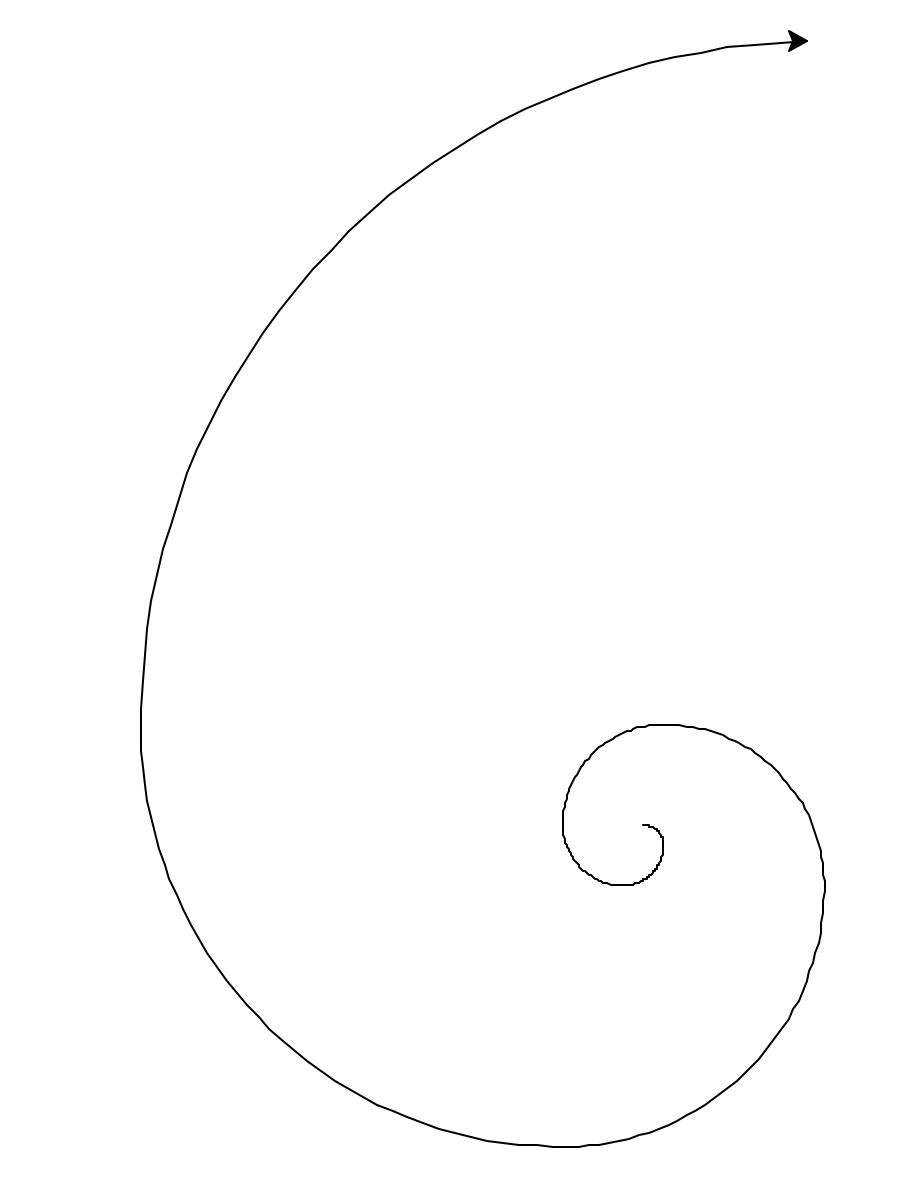
\includegraphics[width=0.35\linewidth]{Grundlagen_Info/00_Programmieren/Skript/Figures/Fibonacci}
		\caption{Fibonacci-Spirale}
		\label{fig:fibonacci}
	\end{figure}

	\begin{myanswer}
		\lstinputlisting[language=Python,caption=\texttt{challenge\_fib.py},label=listing:challenge_fib]{Grundlagen_Info/00_Programmieren/Skript/Code/K03_Variables_Debugging/challenge_fib.py}
	\end{myanswer}
\end{mychallenge}
